\chapter{Threads \& Concurrency}

\section{Process Concept}

Task, process and subprocess are all synonym. We talked about how to fork a process, parent con create a child a copy of the parent. They are two different process with one signle thread each.

We also sad that when we switch from process to another the context switch must copy all the data (registers, PC, code, opened files, etc.) and this require time and more small it is more efficient are the OS.

So is not efficient to duplicate all the parent instead of a small part of process.
\paragraph{}
We would like to reduce this overhead to improve overall performance and the solution is to use \textbf{thread}. 

\subsection{Motivation}

Most, may be all, modern application are multithreaded, thread run within application. Multiple tasks, in a single application, can be implemented by separated threads:
\begin{itemize}
    \item Update display;
    \item Fetch data from file/network;
    \item Spell checking;
    \item Send data into the net;
    \item etc.
\end{itemize}

Also they can simplify code and increase efficiency also kernel are generally multithreaded.
\paragraph{}
Another big difference is: process creation is \textbf{heavy-weight}, like I sad before, while thread creation is \textbf{light-weight}.

\newpage

\section{Multi-Threading}

\subsubsection{Single and Multithreaded processes}

\textbf{Thread} is a basic unit of CPU usage composed of \textbf{thrID}, \textbf{PC}, \textbf{register set}, \textbf{stack} and some shared data: \textbf{heap data}, \textbf{code} (text) and \textbf{OS resouces} with other threads belonging to the same process.

\begin{figure}[htbp]
    \centering
    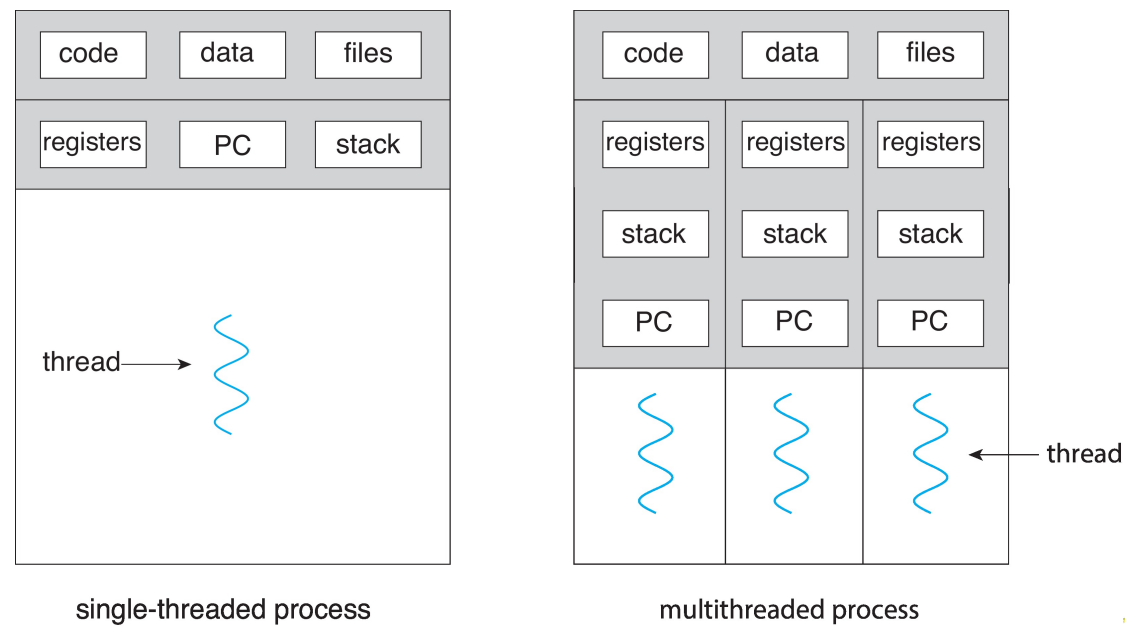
\includegraphics[width=0.65\linewidth]{img/threads.png}   
\end{figure}

Example:
\begin{figure}[htbp]
    \centering
    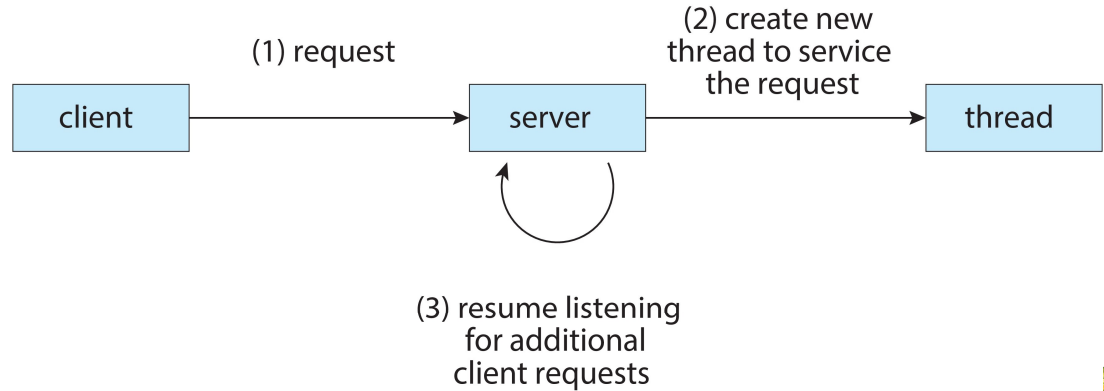
\includegraphics[width=0.65\linewidth]{img/thread_EX.png}   
    
\end{figure}



\subsection{Fork == Thread?}
At this point, you may ask yourselves if the UNIX fork spawns a \textbf{new process} (child of the caller) or a \textbf{Thread}? The answer is: it spawns a child process.

But then, what is the difference between a child process and a thread?

\subsection{Linux Threads}
For Linux systems refers to them as \textbf{tasks} rather than \textbf{threads}.

Task (process) creation is done through \textit{fork()} but also Task (thread) creation is done through \textit{clone()} system call. This function, depends on the parameters passed, can allows a child task to share the address spaces of the parent task (process).

Flags control behavior, can be used for both:

\begin{figure}[htbp]
    \centering
    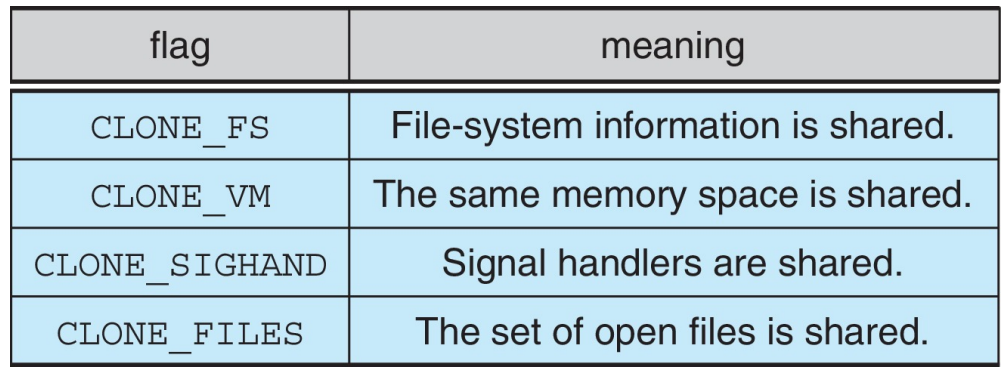
\includegraphics[width=0.55\linewidth]{img/flags.png}
    \caption{Flags to use in clone}    
\end{figure}

\newpage
By default:
\begin{itemize}
    \item fork copies all data structures of the parent process to the child,
    \item while clone points to them
\end{itemize}

\subsubsection{Fork child processes:}
Are processes, so its creation is heavier than threads, the purpose is to create a new process, which becomes the child
process of the caller. Both processes will execute the next instruction following the \textit{fork()} system call and if the child wants to communicate with the parent, it has to set-up brand new shared memories or message-passing because if the parents change the value of a variable the child does not see it (because is a copy).

Two identical copies of the computer's address space,code, and stack are created one for parent and child. Like "Dolly" sheep.


\subsubsection{Threads:}
Purpose is to create a new thread in the program which is given the same process of the caller and threads within the same process can communicate using
shared memory.

The second thread will share data, open files, signal handlers
and signal dispositions, current working directory, user and
group ID's. The new thread will get its own stack, thread ID,
and registers though.

Continuing the analogy: if it was a sheep, your process grows a
fifth head or a second tail when it creates a new thread; those are
connected and share the same brain.


\subsubsection{In my OS}

But then, is my OS scheduling processes or threads?

\begin{itemize}
    \item The Linux scheduler (on recent Linux kernels, e.g. 3.0 at least) is scheduling schedulable tasks or “ready” tasks. 
    \item A task/job may be: 
        \begin{itemize}
            \item[]a single-threaded process (e.g. the main of a C code, or something
created by fork without any thread library);
            \item[] any thread inside a multi-threaded process (including its main
thread), in particular Posix threads;
            \item[] kernel tasks, which are started internally in the kernel and stay in
kernel land (e.g. kworker, nfsiod, kjournald …). These are managed directly by the OS.
        \end{itemize}
\end{itemize}

In other words, threads inside multi-threaded processes are scheduled
like non-threaded -i.e. single threaded- processes.

\section{Benefits}
Using threads improve the overall OS this is some resons:
\begin{itemize}
    \item \textbf{Responsiveness} -- may allow continued execution if part of
    process is blocked, especially important for user interfaces;
    
    \item \textbf{Resource Sharing} -- threads share resources of process, easier
    than shared memory or message passing;
    
    \item \textbf{Economy} -- cheaper than process creation, thread switching
        lower overhead than context switching: \textbf{Don’t need to resent} the cache/CPU is I am switching from a
        process thread to another thread of the same process;
        
    \item \textbf{Scalability} -- process can take advantage of multicore
    architectures: This is true also for single-threaded processes if handled
correctly.
\end{itemize}

\newpage
\section{Multicore Programming}

Multicore or multiprocessor systems put pressure on programmers,
challenges include:

\begin{itemize}
    \item[] Dividing activities
    \item[] Balance load
    \item[] Data splitting
    \item[] Data dependency
    \item[] Testing and debugging
\end{itemize}


\paragraph{Concurrency: } supports more than one task making progress. Single processor / core, scheduler providing concurrency.
\begin{figure}[htbp]
    \centering
    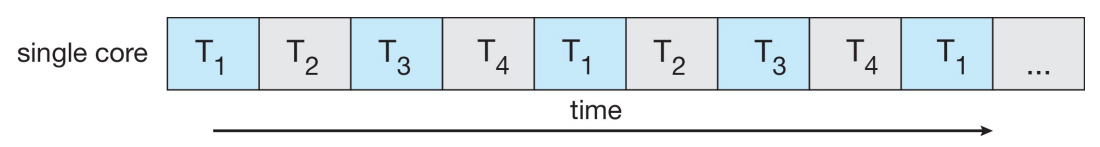
\includegraphics[width=0.7\linewidth]{img/CONCURRENT.png}
    \caption{Concurrent execution on single-core system}
    
\end{figure}
Not really concurrent, there is still at most a thread executing at once. However, it gives the impression that many things are running in
parallel.

If there are lots of process the time between the first and the last are more relevant.
\paragraph{}

\paragraph{Parallelism: } implies a system can perform more than one task simultaneously.

\begin{figure}[htbp]
    \centering
    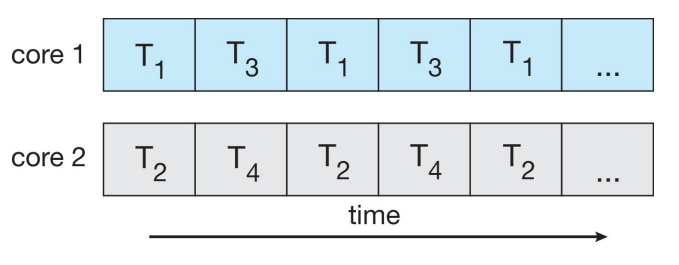
\includegraphics[width=0.45\linewidth]{parallel_exe.png}
    \caption{Parallel execution on a multi-core system}    
\end{figure}

The are two type of parallelism:

\begin{itemize}
    \item -- \textbf{Data parallelism:} distributes subsets of the same data
across multiple cores, same operation on each, none data is shared with other tasks;
        \begin{itemize}
            \item[] e.g. quicksort, margesort.
        \end{itemize}
    \item -- \textbf{Task parallelism:} distributing threads across cores, each
thread performing \textbf{unique operation}, you have some data that it can be shared in different tasks.
        \begin{itemize}
            \item[] e.g. pipelining
        \end{itemize}
\end{itemize}

\begin{figure}[htbp]
    \centering
    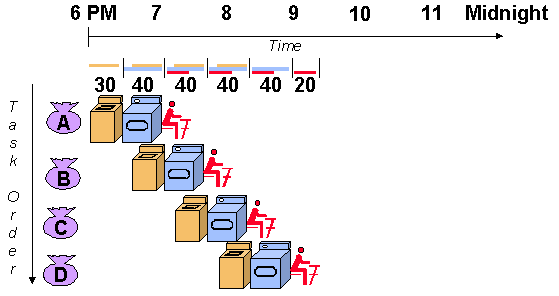
\includegraphics[width=0.65\linewidth]{img/pipeling.png}
    \caption{Pipelining}    
\end{figure}

\newpage
Pipelining, a standard feature in RISC processors, is much like an assembly line. Because the processor works on different steps of the instruction at the same time, more instructions can be executed in a shorter period of time.


\paragraph{RISC Pipelines:} A RISC processor pipeline operates in much the same way, although the stages in the pipeline are different. While different processors have different numbers of steps, they are basically variations of these five, used in the MIPS R3000 processor:

\begin{enumerate}
    \item fetch instructions from memory
    \item read registers and decode the instruction
    \item execute the instruction or calculate an address
    \item access an operand in data memory
    \item write the result into a register
\end{enumerate}

\begin{figure}[htbp]
    \centering
    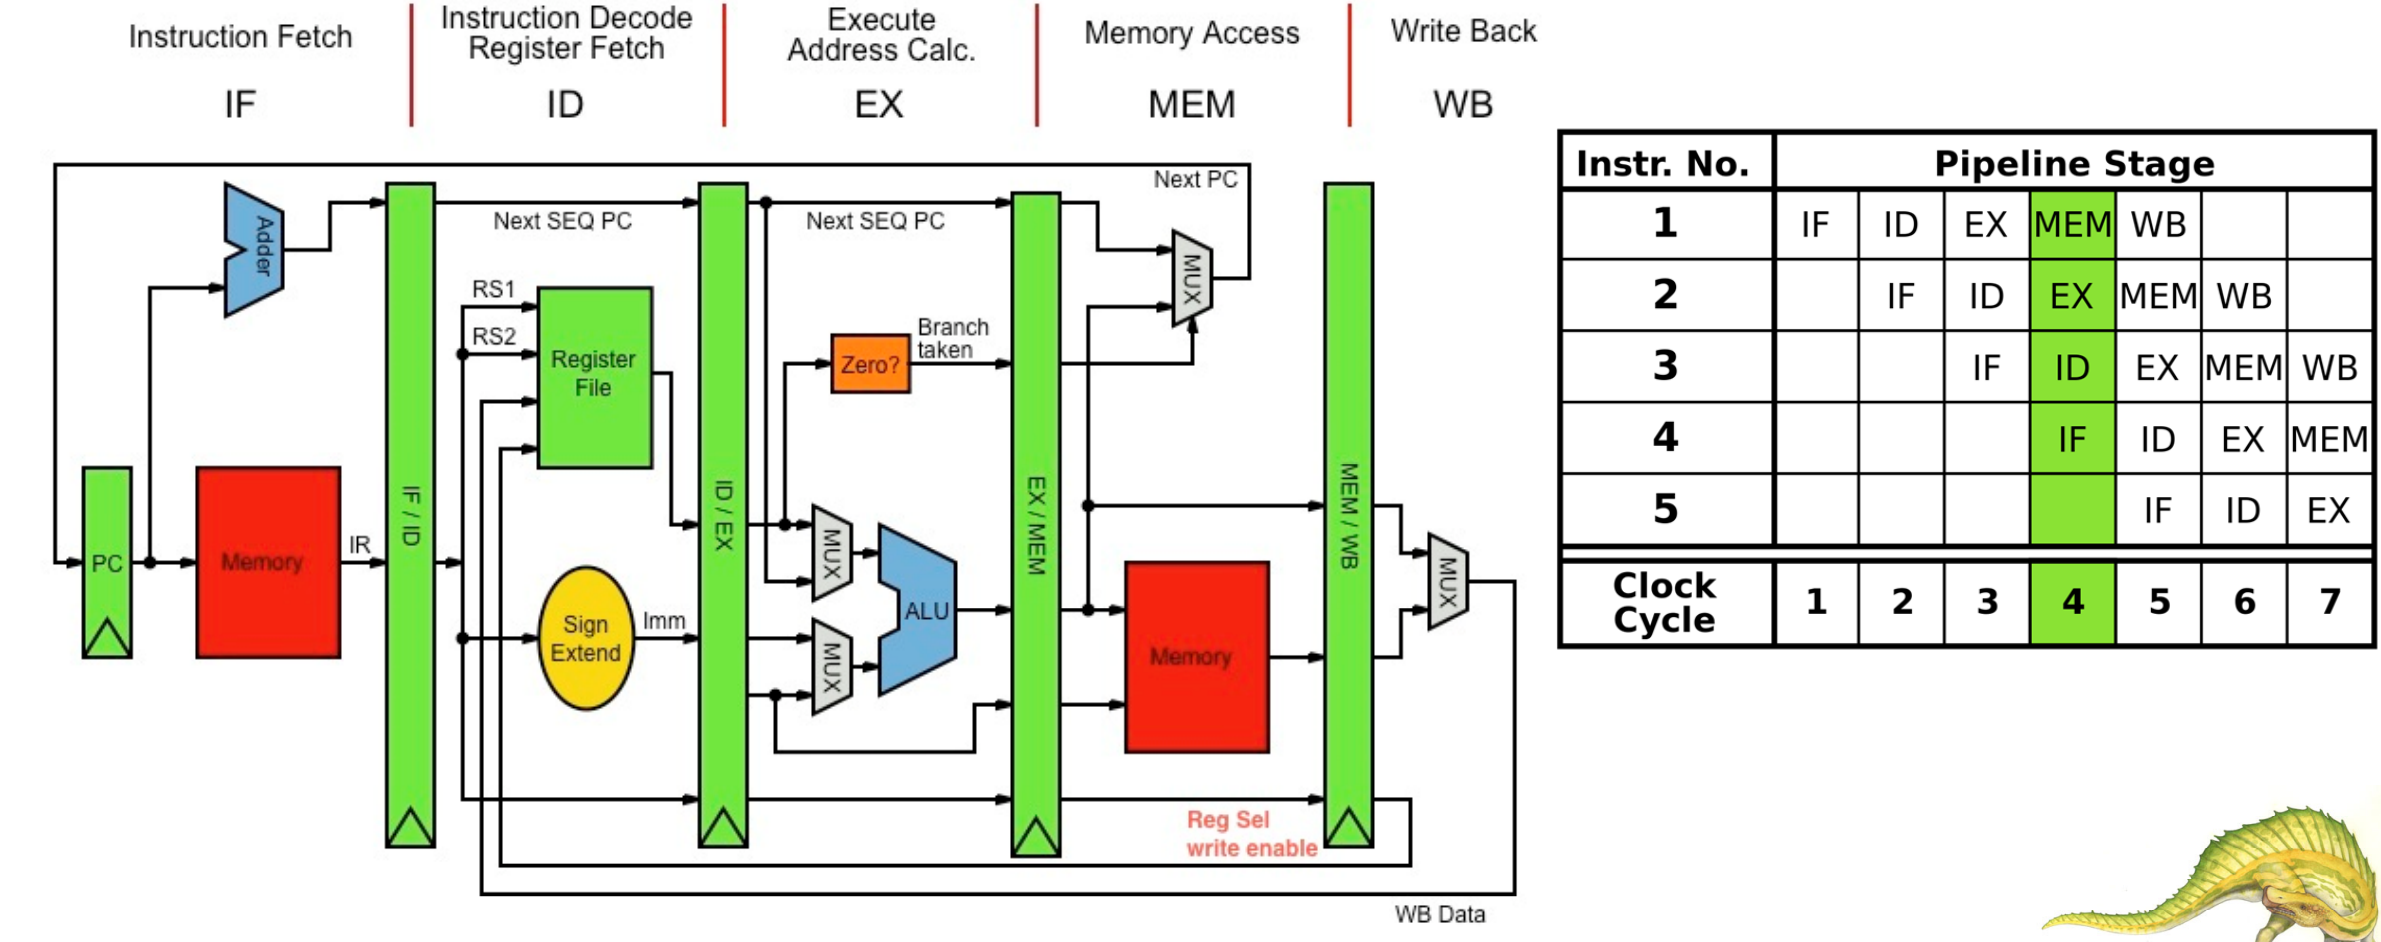
\includegraphics[width=0.8\linewidth]{img/ALU.png}    
    \caption{ALU}
\end{figure}


\newpage
\section{Amdahl’s Law}

Identifies performance gains from adding additional cores (\textbf{N}) to an application that has both serial (\textbf{S}) and parallel (\textbf{P}) components.

\begin{equation*}
    \textit{speedup} \leq \frac{1}{S+\frac{1-S}{N}}
\end{equation*}

That is, if application is $75\%$ parallel / $25\% $ serial, moving from 1 to 2
cores results in speedup of 1.6 times, so not the x2 improvement.

As N approaches infinity, speedup approaches 1/S and if S approaches 1 the speedup approaches 1 (no speedup).

\begin{figure}[htbp]
    \centering
    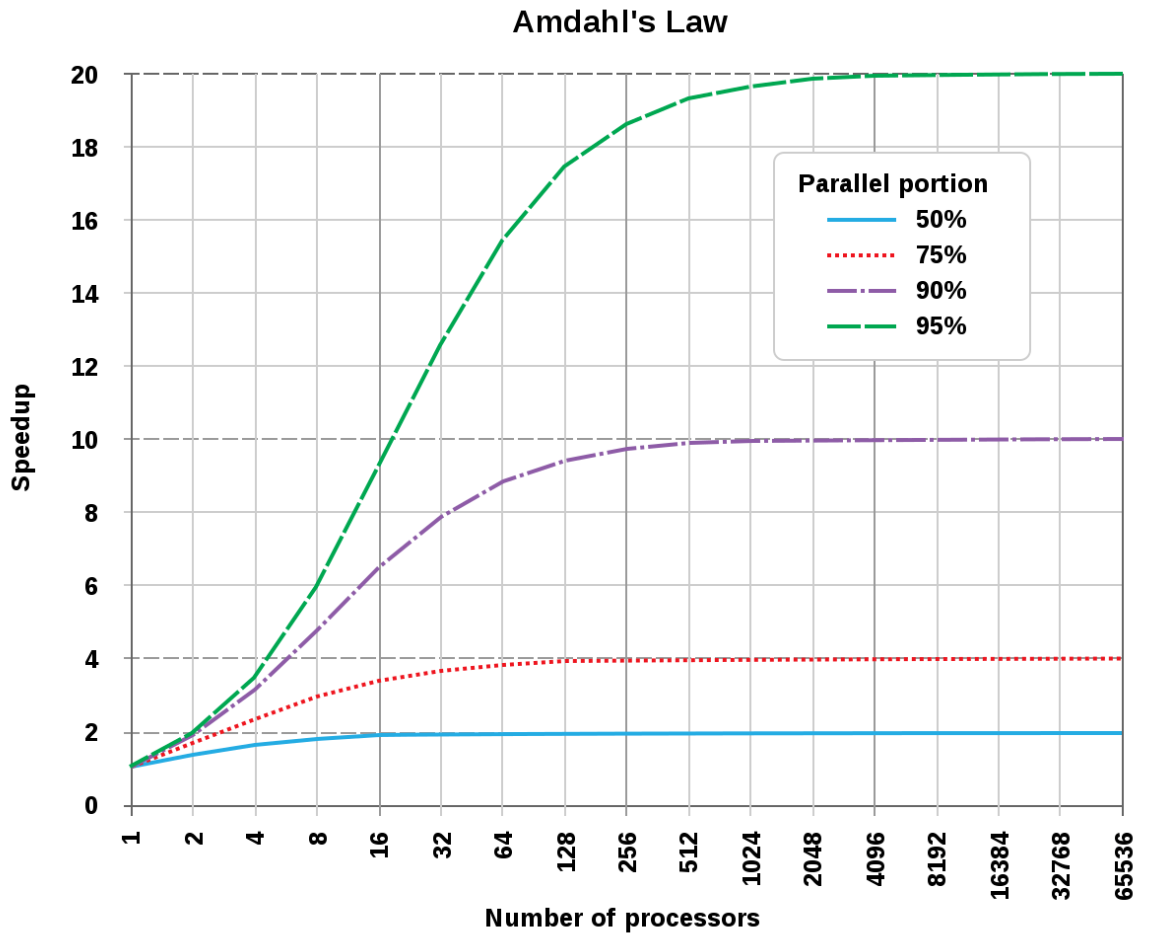
\includegraphics[width=0.65\linewidth]{img/amdahl'slaw.png}
    \caption{Amdahl’s Law}    
\end{figure}

\newpage
\section{Multi-thread models}

It could be dangerous to create a lot of threads, think about a virus that create lots of threads doing nothing only steel time CPU of others processes.

There are two different threads: 

\begin{itemize}
    \item[] \textbf{User thread} -- management done by user-level threads library (pthread, Windows thread, Java runnables and threads)
    \item[] \textbf{Kernel threads} -- Supported by the Kernel
\end{itemize}

\begin{figure}[htbp]
    \centering
    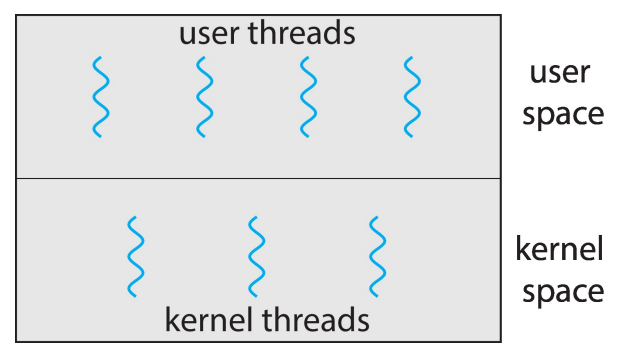
\includegraphics[width=0.5\linewidth]{img/user_space_thread.png}    
\end{figure}

The OS maps user and kernel thread in three way:

\begin{itemize}
    \item Many-to-One
    \item One-to-One
    \item Many-to-Many
\end{itemize}

\subsection{Many-to-One}

Many user-level threads mapped to single kernel thread, multiple threads may not run in parallel on multicore system because
only one may be in kernel at a time.

If one thread blocking causes all to block. This approach is use in a few OS like Solaris Green Threads or GNU Portable Threads.

\begin{figure}[htbp]
    \centering
    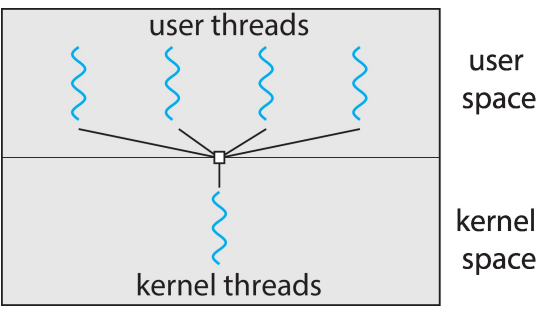
\includegraphics[width=0.5\linewidth]{img/MtM.png}
    \caption{Many-to-One thread}    
\end{figure}

\newpage
\subsection{One-to-One}

The easiest solution, each user-level thread maps to kernel thread this allows to more concurrency than many-to-one.

For the security the number of threads per process sometimes restricted due to overhead.

Some example are: \textbf{Windows} and \textbf{Linux} systems.

\begin{figure}[htbp]
    \centering
    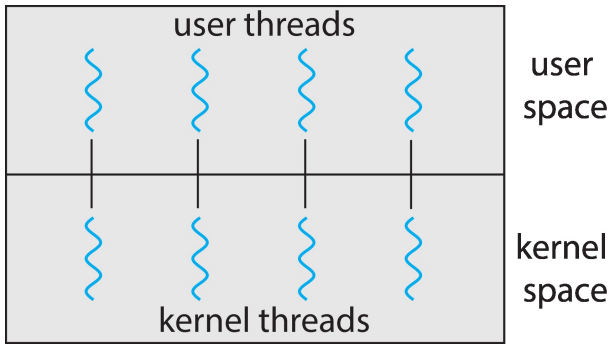
\includegraphics[width=0.5\linewidth]{img/OtO.png}
    \caption{One-to-One thread}    
\end{figure}

\subsection{Many-to-Many}
The last solution is a mix of the approach talked before.

Allows many user level threads to be mapped to many kernel threads if I have N user threads, I will be mapped into M ($\leq$ N) kernel threads this M size can be set by the OS, also considering the amount of
available cores, or the amount of processes allows the operating system to create a sufficient number of kernel
threads without over-creating them

Very complex to implement and manage.

Some example are: Windows with the ThreadFiber package, otherwise not very common.

\begin{figure}[htbp]
    \centering
    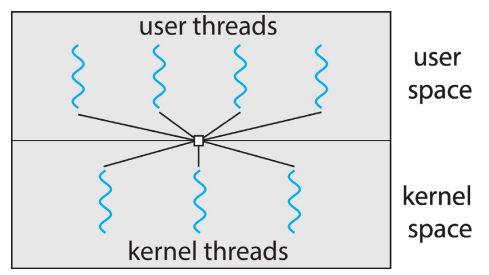
\includegraphics[width=0.5\linewidth]{img/MtMM.png}
    \caption{Many-to-Many thread}        
\end{figure}

\newpage
\subsection{Two-level Model: } similar to many-to-many, except that it allows a user thread to be bound to kernel thread. Not really used in practice.

\begin{figure}[htbp]
    \centering
    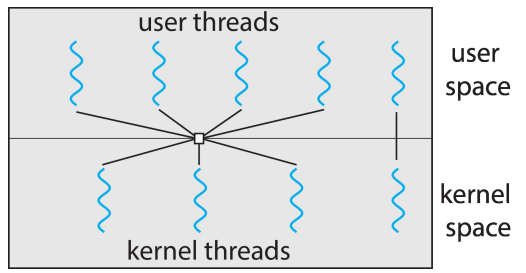
\includegraphics[width=0.5\linewidth]{img/TlT.png}
    \caption{Two-level Model}
    
\end{figure}

\newpage
\section{Thread libraries}
A Thread library provides programmer with API for creating and managing threads. Two primary ways of implementing: Library entirely in user space; Kernel-level library supported by the OS.

\subsubsection{Pthreads}
A POSIX standard (IEEE 1003.1c) API for thread creation and synchronization, is a Specification, not implementation. Infact API specifies behavior of the thread library, implementation is up to development of the library, this is common in UNIX OS (Linux and Mac OS X).
\paragraph{}
There are around 100 threads procedures, all prefixed pthread$\_$ and
they can be categorized into four groups:

\begin{itemize}
    \item Thread management – creating, joining threads etc.
    \item Mutexes
    \item Condition variables
    \item Synchronization between threads using read write locks and
barriers
    \item  Spinlocks
\end{itemize}


\subsubsection{Pthread\_attr\_init}

Initializes thread attributes, needed for creating new threads, by default it creates a structure like:

\begin{itemize}
    \item[] Detach state = PTHREAD\_CREATE\_JOINABLE 
    \item[] Scope = PTHREAD\_SCOPE\_SYSTEM
    \item[] Inherit scheduler = PTHREAD\_INHERIT\_SCHED
    \item[] Scheduling policy = SCHED\_OTHER
    \item[] Scheduling priority = 0
    \item[] Guard size = 4096 bytes
    \item[] Stack address = 0x40196000
    \item[] Stack size = 0x201000 bytes
\end{itemize}


\subsubsection{Pthread\_create}

Creates a new thread, initializing its tid, the function required some inputs:
\begin{itemize}
    \item The empty tid value (need to pass the address – by reference);
    \item The thread attributes (pass by reference, again);
    \item A pointer to the function to be exercised by the thread;
    \item Params of the function, as specified in the signature.
\end{itemize}

\begin{codeInC}
int pthread_create( pthread_t *restrict thread,
                    const pthread_attr_t *restrict attr,
                    void *(*start_routine)(void *),
                    void *restrict arg );
\end{codeInC}

In Linux when you call the create() function it means, create and run the thread.


\subsubsection{Pthread\_join}

The pthread\_join() function waits for the thread specified by thread to
terminate. If that thread has already terminated, then pthread\_join()
returns immediately. The thread specified by thread must be joinable.

Means that if a process calls the pthread\_join and the thread never
ends (stuck somewhere, …) the process will wait endlessly, it is called a \textbf{blocking function call}.

\begin{codeInC}
int pthread_join(pthread_t thread, void **retval);
\end{codeInC}

\subsubsection{Pthread\_exit}

The pthread\_exit() function terminates the calling thread and returns a
value via retval that (if the thread is joinable) is available to another
thread in the same process that calls pthread\_join().

To access the return value you have to provide a non-NULL pointer as
a second parameter of the pthread\_join function, this has to be typed as a void**.


\begin{codeInC}
[[noreturn]] void pthread_exit(void *retval);
\end{codeInC}

\paragraph{}
\textbf{Example: }


\begin{codeInC}

#include <pthread.h>
#include <stdio.h>

#include <stdlib.h>

int sum; /* this data is shared by the thread(s) */
void *runner (void *param); /* threads call this function */

int main(int argc, char *argv[]) {

    pthread_t tid; /* set the thread identifier */
    pthread_attr_t attr; /* set of thread attributes */
    
    /* set the default attributes of the thread */
    pthread_attr_init(&attr);
    /* create the thread */    
    pthread_create(&tid, &attr, runner, argv[1]);
    /* wait for the thread to exit */    
    pthread_join(tid, NULL);
    
    printf("sum = %d\n", sum);
}


/* The thread will execute in this function */
void *runner (void *param){

    int i, upper = atoi(param);
    sum = 0;
    
    for (i=1; i <= upper; i++)
        sum += i;
    
    pthread_exit(0);
}
\end{codeInC}


\subsection{JAVA THREADS}

When you write code in Java therads are managed by the JVM, typically implemented using threads model provided by underlying OS.

\paragraph{NOTE:} the JVM is a middlewere between your code and the host OS, thus uses OS-specific funztions.
\paragraph{}
Java thread may be created by:

\begin{itemize}
    \item Extending Thread class;
    \item Implementing the Runnable interface;
\end{itemize}

The standard practise to implement thread is to implement the \textbf{Runnable interface}:

\begin{codeInJava}
class Task implements Runnable{

    ...
    
    public void run(){
        System.out.println("I am a thread.");
    }

    ...
}

\end{codeInJava}

creation and waiting on a thread:

\begin{codeInJava}
import java.lang.Thread;

class Main {

    public static void main() {

        Thread worker = new Thread(new Task());
        worker.start();

        try{
            worker.join();
        }catch(InterruptedException ie){
            System.out.println("An error occurred.");
        }
        
    }
}
\end{codeInJava}

\newpage
\subsection{OpenMP}

In C, the process of creating a thread costs a lot of time and effort to the programmer. For this reason openMP libraries automatically implement the creation and the waiting.

Is a set of compiler directives and an API for C, C++, FORTRAN; it provides support for parallel
programming in shared-memory environments and identifies \textbf{parallel regions} – blocks of code that can run in
parallel. 
All of this only writing a single line: \verb|#pragma omp parallel|, it create as many threads as there are cores.

\begin{codeInC}
#include <omp.h>
#include <stdio.h>

int main(int argc, char *argv[]) {

    /* sequential code */
    
    #pragma omp parallel
    {                           //you must go to the new line
        printf("I am a parallel region.");
    }
    
    
    /* sequential code */
    
    return 0;
}
\end{codeInC}
\paragraph{}
There are different ways to make parallel code with omp, the code above defines a parallel region, which is code that will be executed by multiple threads in parallel, to enforce a given number of threads you should disable dynamic teams and specify the desired number of threads with either \verb|omp_set_num_threads()|:
\paragraph{}
\begin{codeInC}
#include <omp.h>

omp_set_dynamic(0);     // Explicitly disable dynamic teams
omp_set_num_threads(4); // Use 4 threads for all consecutive parallel regions

#pragma omp parallel ...
{
  // Code here will be run by 4 threads in parallel
}


\end{codeInC}
\paragraph{}
Or with the \verb|num_threads| OpenMP clause:
\paragraph{}
\begin{codeInC}
omp_set_dynamic(0);     // Explicitly disable dynamic teams
// Spawn 4 threads for this parallel region only

#pragma omp parallel... num_threads (4)
{
  // Code here will be run by 4 threads in parallel
}

\end{codeInC}

\newpage
\subsubsection{Directives}
There are different ways to make parallel code with omp.

\begin{itemize}
    \item \textbf{Pragma omp parallel } 
    \begin{itemize}
        \item[] Defines a parallel region, which is code that will be executed by multiple threads in parallel.
    \end{itemize}

    \item \textbf{Pragma omp for } 
    \begin{itemize}
        \item[] Causes the work done in a for loop inside a parallel region to be divided among threads.
    \end{itemize}

    \item \textbf{Pragma omp sections } 
    \begin{itemize}
        \item[] Identifies code sections to be divided among all threads.
        \item[] Each section has to be tagged as pragma omp section.
    \end{itemize}

    \item \textbf{Pragma omp single } 
    \begin{itemize}
        \item[] Lets you specify that a section of code should be executed on a single thread, not necessarily the main thread.
    \end{itemize}
\end{itemize}

If I only have one line of code within a parallel block, I just mark the single line with the last directives above.

\begin{codeInC}

int main(){

    ...

    #pragma omp parallel
    {

        //parallel

        #pragma omp single
        {
            // sequential
        }
        
        //parallel
    
    }

    return 0;
}
    
\end{codeInC}


\newpage
\section{Implicit threading}

Growing in popularity as numbers of threads increase, program correctness more difficult with explicit threads. Creation and management of threads done by compilers and run-time libraries rather than programmers (e.g. OpenMP).

This is called implicit threading, because the creation and all the waiting mechanisms of the thread are managed in the background.

\paragraph{Some methods to use implicit thread:}
\begin{itemize}
    \item Thread Pools
    \item Fork-Join
    \item OpenMP
    \item Grand Central Dispatch
    \item Intel Threading Building Blocks
\end{itemize}

\subsection{Thread Pools}

This library emulate OpenMP in Java language, it crate  a number of threads in a pool where they await work.

\paragraph{Some advantages:}

\begin{itemize}
    \item Usually slightly faster to service a request with an existing thread than create a new thread
    \item Allows the number of threads in the application(s) to be bound to the size of the pool
    \item Separating task to be performed from mechanics of creating task allows different strategies for running task
        \begin{itemize}
            \item[] E.g. Tasks could be scheduled to run periodically
        \end{itemize}
\end{itemize}

Three factory methods for creating thread pools in Executors class:

\begin{codeInJava}
static ExecutorService newSingleThreadExecutor();
static ExecutorService newFixedThreadPool(int size);
static ExecutorService newCachedThreadPool();
    
\end{codeInJava}


\paragraph{Example:}

\begin{codeInJava}
import java.util.concurrent.*;

public class ThreadPoolExample {

    public static void main(String[] args) {
    
        int numTasks = Integer.parseInt(args[0].trim());
        
        /* Create the thread pool */
        ExecutorService pool = Executors.newCachedThreadPool();
        
        /* Run each task using a thread in the pool */
        for (int i = 0; i < numTasks; i++)        
            pool.execute(new Task());
        
        /* Shut down the pool once all threads have completed */
        pool.shutdown();    
    }
}
    
\end{codeInJava}
\newpage

But also Windows API supports thread pools:

\begin{codeInJava}
DWORD WINAPI PoolFunction(AVOID Param){
    /*
    * This function runs as a separated thread.
    */
}
    
\end{codeInJava}


\subsection{Fork-Join Parallelism}

Multiple threads (tasks) are forked, and then joined, this allows to emulate parallelism (not threads) because it is a sub-process. Creation of sub-process is a heavy operation instead to create threads, also each fork have a copy of memory and not shared memory.

\begin{figure}[htbp]
    \centering
    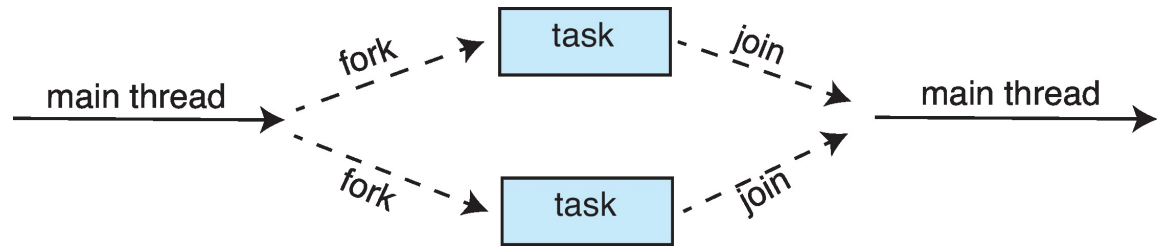
\includegraphics[width=0.7\linewidth]{img/fork_join.png}
\end{figure}

\paragraph{General algorithm for fork-join strategy:}

\begin{codeInC}
Task(problem)   

if problem is small enough 
    then 
        solve the problem directly 
else
    then
        subtask1 = fork(new Task(subset of problem))                
        subtask2 = fork(new Task(subset of problem))                
        result1 = join(subtask1)                                        
        result2 = join(subtask2)   
endif

return combined results                                    

\end{codeInC}

\begin{figure}[htbp]
    \centering
    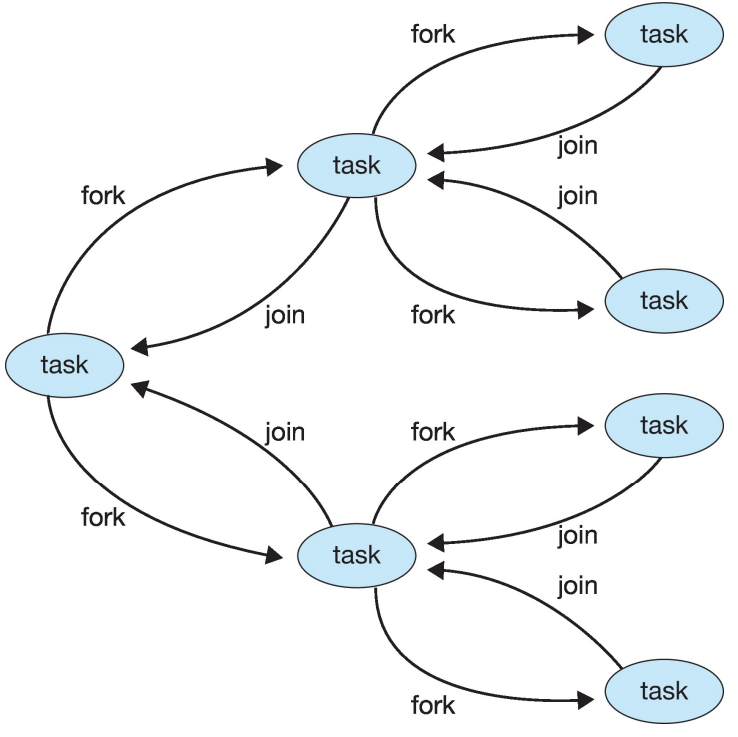
\includegraphics[width=0.5\linewidth]{img/F_J_parall.png}
    \caption{Fork-Join Parallelism state machine}    
\end{figure}





